
\chapter{恒等式}
\label{chap:identities}

\section{基本恒等式}
\label{sec:basic-identities}

\begin{example}
  $\forall n\in\mathbb{Z^+}$,有$(1+2+3+\cdots+n)^2 = 1^3 + 2^3 + \cdots + n^3$,即
  \begin{align*}
    \left(\sum_{x=1}^n x \right)^2 = \sum_{x=1}^n x^3
  \end{align*}
\end{example}
\begin{proof}[提示]归纳。
  \begin{align*}
    \left(\sum_{x=1}^{n+1} x \right)^2 ={}& \left((n+1) + \sum_{x=1}^{n} x \right)^2 \\
    ={}& (n+1)^2 + 2(n+1)\left(\sum_{x=1}^{n} x \right) + \left(\sum_{x=1}^{n} x \right)^2\\
    ={}& (n+1)^2 + 2(n+1)\cdot\frac{n(n+1)}{2} + \sum_{x=1}^n x^3\\
    ={}& (n+1)^3 + \sum_{x=1}^n x^3
  \end{align*}
\end{proof}


\begin{example}[两数和的幂]$\forall a,b\in\mathcal{R}$,有
  \begin{align*}
    (a + b)^2 &= a^2 + 2ab + b^2\\
    (a + b)^3 &= a^3 + 3a^2b + 3ab^2 + b^3\\
    (a + b)^4 &= a^4 + 4a^3b + 6a^2b^2 + 4ab^3 + b^4
  \end{align*}
\end{example}
对于$(a-b)^2$及$(a-b)^3$这种,只要在上式中把$b$换为$-b$即可。观察上述$(a+b)^n$的系数,可以发现其与下面的杨辉三角是一致的:
\begin{center}
  \begin{tikzpicture}[scale=1.0]
    \begin{scope}[shift={(.5,1)}]
      \foreach \x/\v in {1/1,2/1}{%
        \node at (\x,0) {\v};
      }
    \end{scope}
    \begin{scope}[shift={(0,0)}]
      \foreach \x/\v in {1/1,2/2,3/1}{%
        \node at (\x,0) {\v};
      }
    \end{scope}
    \begin{scope}[shift={(-.5,-1)}]
      \foreach \x/\v in {1/1,2/3,3/3,4/1}{%
        \node at (\x,0) {\v};
      }
    \end{scope}
    \begin{scope}[shift={(-1,-2)}]
      \foreach \x/\v in {1/1,2/4,3/6,4/4,5/1}{%
        \node at (\x,0) {\v};
      }
    \end{scope}
    \begin{scope}[shift={(-1.5,-3)}]
      \foreach \x/\v in {1/1,2/5,3/10,4/10,5/5,6/1}{%
        \node at (\x,0) {\v};
      }
    \end{scope}
    \foreach \y in{1,2,3,4,5}{%
      \node[left] at (-2,2-\y){$n=\y$};
    }
  \end{tikzpicture}
\end{center}


\begin{example}[配方]$\forall a\ne 0$,有
  \begin{align*}
    ax^2 + bx + c = a\left(x-\frac{b}{2a}\right)^2 + \frac{4ac - b^2}{4a}
  \end{align*}
\end{example}

\section{代数}
\label{sec:algebra-identities}

\begin{theorem}[Sophie-Germain恒等式]
  $\forall x,y$,有
  \begin{align*}
    x^4 + 4y^4 = (x^2 + 2xy + 2y^2)(x^2 - 2xy + 2y^2)
  \end{align*}
\end{theorem}
在上式中令$x=1$,可以得到哥德巴赫定理;令$y=1$,则可以得到吉梅茵定理。
\begin{theorem}[哥德巴赫定理,Goldbach Theorem]\mbox{}\par
  对任意整数$n>1$,$4n^4+1=(1+2n+2n^2)(1-2n+2n^2)$是合数。  
\end{theorem}
\begin{theorem}[吉梅茵定理,Germain Theorem]\mbox{}\par
  任意整数$n>1$,$n^4+4=(n^2+2n+2)(n^2-2n+2)$是合数。
\end{theorem}


\begin{theorem}[贝祖定理,B\'ezout's identity]\label{th:Bezout}
  $\forall a,b\in\mathcal{Z},\exists x,y\in\mathcal{Z}$使得
  \begin{align*}
    ax+by=\mathrm{gcd}(a,b)
  \end{align*}
  若$a,b$互质,则有$ax+by=1$。
\end{theorem}

\begin{theorem}\label{th:inverse-bezout}
  若整数$x,y,a,b$满足$ax+by=1$,则$x,y$互质。从而$\gcd(a,b)=\gcd(a,y)=\gcd(x,b)=\gcd(x,y)=1$。
\end{theorem}
\begin{proof}
  记$g=\gcd(x,y)$,则$x'=x/g$与$y'=y/g$是互质的两个整数,代入有
  \begin{align*}
    1=ax+by=ax'g+by'g=g(ax'+by')
  \end{align*}
  从而$g\mid 1\implies g=1$。
\end{proof}

%%% $x,y$称为$(a,b)$的B\'ezout系数。一般来说,$(a,b)$的B\'ezout系数$x,y$不是唯一的,可以通过扩展欧几里得算法来计算得到。
$x,y$称为$(a,b)$的B\'ezout系数。一般来说,$(a,b)$的B\'ezout系数$x,y$不是唯一的,可以通过类似于欧几里得辗转相除法得到。

\begin{example}
  求整数$a,b$使得$211a+37b=1$。
\end{example}
\begin{proof}[提示]
\begin{align*}
  211a+37b=1 &\iff 37b=1-211a \\
             &\iff b=\frac{1-211a}{37}=-5a+\frac{1-26a}{37}\\
             &\iff b=-6a+\frac{1+11a}{37} 
\end{align*}
令$1+11a=37t_1$,其中$t_1$为整数,从而
\begin{align*}
  1+11a=37t_1 & \iff a=\frac{37t_1-1}{11}=3t_1 + \frac{4t_1-1}{11}
\end{align*}
令$4t_1-1=11t_2$,其中$t_2$为整数,则$t_1=2t_2+(3t_2+1)/4$。若能观察出来取$t_2=1$可使$t_1$为整数,则代入即可。

若观察不出来,继续令$3t_2+1=4t_3$,则$t_2=t_3+(t_3-1)/3$,若还观察不出来$t_3$应取什么值可使$t_2$为整数,继续令$t_3-1=3t_4$,从而$t_3=3t_4+1$,整数$t_4$可随意挑选,再一步步反向代入,可得$t_3,t_2,t_1,a,b$。
\end{proof}


% \begin{definition}[扩展欧几里得算法]
%   Ref. \verb|https://en.wikipedia.org/wiki/Extended_Euclidean_algorithm|
% \end{definition}

\begin{example}[1959 IMO]
  求证对任意正整数$n$,分数$\dfrac{21n+4}{14n+3}$不可约。
\end{example}
\begin{proof}[提示]
  相当于证明$21n+4$与$14n+3$互质。尝试使用定理\ref{th:inverse-bezout},若能找到两个整数$a,b$,使得$a(21n+4)+b(14n+3)=1$,则有$21n+4$与$14n+3$互质。而
  \begin{align*}
    a(21n+4)+b(14n+3)=1 \iff (21a + 14b)n + 4a + 3b = 1
  \end{align*}
  而上式要对任意整数$n$成立,等价于以下两式同时成立
  \begin{align*}
    21a+14b=0, \quad 4a+3b=1
  \end{align*}
  而这个方程组是有整数解$a=-2, b=3$,从而原问题得证。
\end{proof}

\begin{example}\label{ex:sum-is-negative-to-product}
  对任意满足$a+b\ne0$,$b+c\ne0$,$c+a\ne0$的实数$a,b,c$,则以下三个数的和与积互为相反数:
  \begin{align*}
    \frac{a-b}{a+b},\quad \frac{b-c}{b+c},\quad \frac{c-a}{c+a}
  \end{align*}
  即
  \begin{align*}
    \frac{a-b}{a+b} + \frac{b-c}{b+c} + \frac{c-a}{c+a} 
    + \frac{a-b}{a+b} \cdot \frac{b-c}{b+c} \cdot \frac{c-a}{c+a} = 0
  \end{align*}
\end{example}
\begin{proof}
  记
  \begin{align*}
    S\equiv \frac{a-b}{a+b} + \frac{b-c}{b+c} + \frac{c-a}{c+a}
  \end{align*}
  问题中的等式等价于
  \begin{align*}
    S \cdot (a+b)(b+c)(c+a) = -(a-b)(b-c)(c-a)
  \end{align*}
  最直接的方法,是逐项展开,合并同类项。
  \begin{align*}
       & S\cdot (a+b)(b+c)(c+a)\\
    ={}& \underline{(a-b)(b+c)(c+a)} + \underline{(b-c)(c+a)(a+b)} + (c-a)(a+b)(b+c)\\
    ={}& (c+a)\left( (a-b)(b+c) + (b-c)(a+b) \right) + (c-a)(a+b)(b+c)\\
    ={}& 2b(c+a)(a-c) + (c-a)(a+b)(b+c)\\
    ={}& (a-c)(2bc+2ab - (ab+ac+bb+bc))\\
    ={}& (a-c)(bc+ab - ac-bb)\\
    ={}& (a-c)(c(b-a)+b(a-b))\\
    ={}& (a-c)(b-a)(c-b)\\
    ={}& -(a-b)(b-c)(c-a) &&\qedhere
  \end{align*}
\end{proof}

\begin{example}
  若$a=3,b=4,c=5$,则
  \begin{align*}
    \frac{a-b}{a+b} = \frac{3-4}{3+4} = -\frac17\\
    \frac{b-c}{b+c} = \frac{4-5}{4+5} = -\frac19\\
    \frac{c-a}{c+a} = \frac{5-3}{5+3} = \phantom{-}\frac14
  \end{align*}
  其和为
  \begin{align*}
    -\frac17 - \frac19 + \frac14 = \frac{-9\times4 - 7\times4 + 7\times9}{4\times7\times9} = -\frac1{4\times7\times9}
  \end{align*}
  容易看出,其和为其积的相反数。
\end{example}

\section{重要恒等式}
\label{sec:important-identities}

以下几个恒等式不常见,却是竞赛中的常客。虽无需记忆,但可以留点印象,知道有这么回事,对解题有大帮助。

\begin{example}\label{ex:product-of-four-continuous-integer}
  直接两展开,可知对任意$x\in\mathcal{R}$,有
  \begin{align*}
    x(x+1)(x+2)(x+3)+1=\left( x^2+3x+1\right )^2
  \end{align*}
  从而连续4个整数的积再加1是个完全平方数。换一个形式,则有
  \begin{align*}
    \sqrt{x(x+1)(x+2)(x+3)+1}= x^2+3x+1 = (x + 1)^2 + x
  \end{align*}
\end{example}

\begin{example}
  求$\sqrt{2019\times2020\times2021\times2022+1}-2020^2$。

  在恒等式$\sqrt{x(x+1)(x+2)(x+3)+1}= (x + 1)^2 + x$中令$x=2019$,则有
  $\sqrt{2019\times2020\times2021\times2022+1}-2020^2=2019$。
\end{example}

\begin{theorem}[Fibonacci Identity]任意实数$a,b,c,d$,有恒等式
  \begin{align*}
    \left(a^2+b^2\right)\left(c^2+d^2\right)
    = \left(ac +  bd\right)^2 + \left(ad -  bc\right)^2
    = \left(ac -  bd\right)^2 + \left(ad +  bc\right)^2 
  \end{align*}
\end{theorem}

\section{三角函数恒等式}
\label{sec:trigonometric-identities}

\begin{theorem}\label{th:tan-x+y+z=k.pi}
  若$\alpha, \beta, \gamma$均非$\pi/2$的奇数倍,则
  \begin{align*}
    \alpha+\beta+\gamma = k\pi,(k\in\mathbb{Z}) \iff
    \tan\alpha +\tan\beta+\tan\gamma=\tan\alpha \cdot \tan\beta \cdot \tan\gamma
  \end{align*}
  % 当且仅当$$是$\pi$的整数倍时成立。
\end{theorem}
\begin{proof}[提示]
  利用欧拉定理$e^{ix} = \cos x + i \sin x$,有
  \begin{align*}
    e^{i(\alpha + \beta + \gamma)} ={}& e^{i\alpha}\cdot e^{i\beta}\cdot e^{i\gamma} =\\
    ={}& (\cos\alpha + i\sin\alpha) \cdot (\cos\beta + i\sin\beta) \cdot (\cos\gamma + i\sin\gamma)
  \end{align*}
  由此可以得到其虚部
  \begin{align*}
    &\mathrm{Im}\left(e^{i(\alpha + \beta + \gamma)}\right) \\
    ={}& \sin\alpha\cos\beta\cos\gamma + \cos\alpha\sin\beta\cos\gamma + \cos\alpha\cos\beta\sin\gamma - \sin\alpha\sin\beta\sin\gamma
  \end{align*}
  由$\alpha,\beta,\gamma$不是$\pi/2$的奇数倍,可知
  \begin{align*}
    \cos\alpha\ne0,\quad \cos\beta\ne0,\quad \cos\gamma\ne0
  \end{align*}
  从而有
  \begin{align*}
    \frac{\mathrm{Im}\left(e^{i(\alpha + \beta + \gamma)}\right)}{\cos\alpha\cos\beta\cos\gamma}
    = \tan\alpha + \tan\beta + \tan\gamma - \tan\alpha\tan\beta\tan\gamma
  \end{align*}
  由$\left| e^{i(\alpha + \beta + \gamma)} \right| = 1$,可得
  \begin{align*}
    \alpha + \beta + \gamma = k\pi \iff &
    e^{i(\alpha + \beta + \gamma)} = \pm 1 
    \iff \mathrm{Im}\left(e^{i(\alpha + \beta + \gamma)}\right) = 0\\
    \iff & \tan\alpha + \tan\beta + \tan\gamma = \tan\alpha\tan\beta\tan\gamma\qedhere
  \end{align*}

  % 若$\alpha + \beta + \gamma = k\pi$,则
  % \begin{align*}
  %   e^{i(\alpha + \beta + \gamma)} = -1 \implies & \mathrm{Im}\left(e^{i(\alpha + \beta + \gamma)}\right) = 0\\
  %   \iff & \tan\alpha + \tan\beta + \tan\gamma - \tan\alpha\tan\beta\tan\gamma = 0
  % \end{align*}

  % 反之,若$\tan\alpha + \tan\beta + \tan\gamma - \tan\alpha\tan\beta\tan\gamma = 0$,则
  % \begin{align*}
  %   \mathrm{Im}\left(e^{i(\alpha + \beta + \gamma)}\right) = 0
  %   \iff & \sin(\alpha + \beta + \gamma) = 0\\
  %   \iff & \alpha + \beta + \gamma = k\pi,\quad(k\in\mathcal{Z})&&\qedhere
  % \end{align*}
\end{proof}

\begin{example}
  在定理~\ref{th:tan-x+y+z=k.pi}中,用了复平面单位圆上的两个特殊点,即单位圆与实轴的两个交点。若利用单位圆与虚轴上的两个交点,则可以得到类似的结论。

  \begin{center}
    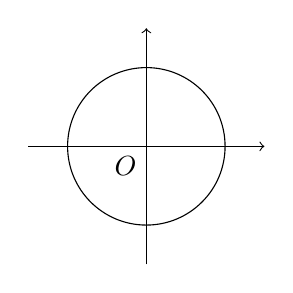
\begin{tikzpicture}[scale=1.0]
      \coordinate(O) at (0,0);
      \coordinate(X1)at(-1,0);\coordinate(X2)at(1,0);
      \coordinate(Y1)at(0,-1);\coordinate(Y2)at(0,1);
      \tkzDrawPoints(O,X1,X2,Y1,Y2)\node[below left]at(O){$O$};
      \draw(O)circle(1);
      \draw[->](-1.5,0)--(1.5,0);
      \draw[->](0,-1.5)--(0,1.5);
    \end{tikzpicture}
  \end{center}
  容易得到单位圆上点的实部的表达式为
  \begin{align*}
        & \mathrm{Re}\left( e^{i(\alpha + \beta + \gamma)}\right) \\
    ={} & \cos\alpha\cos\beta\cos\gamma - \cos\alpha\sin\beta\sin\gamma
          - \sin\alpha\cos\beta\sin\gamma - \sin\alpha\sin\beta\cos\gamma\\
  \end{align*}
  类似定理~\ref{th:tan-x+y+z=k.pi},若$\cos\alpha, \cos\beta, \cos\gamma$均不为0,即$\alpha, \beta, \gamma$均不为$\pi/2$的奇数倍时,有
  \begin{align*}
    \frac{\mathrm{Re}\left( e^{i(\alpha + \beta + \gamma)}\right)}{\cos\alpha\cos\beta\cos\gamma}
    ={} 1 - \tan\alpha\tan\beta - \tan\beta\tan\gamma - \tan\gamma\tan\alpha
  \end{align*}
  取单位圆与虚轴的两个交点,即$\alpha + \beta + \gamma$是$\pi/2$的奇数倍,此两点的实部为0,从而
  \begin{align*}
    \alpha + \beta + \gamma = (2k + 1)\frac\pi2
    \iff & e^{i(\alpha + \beta + \gamma)} = \pm i 
    \iff \mathrm{Re}\left(e^{i(\alpha + \beta + \gamma)}\right) = 0\\
    % \iff & 1 - \tan\alpha\tan\beta - \tan\beta\tan\gamma - \tan\gamma\tan\alpha = 0\\
    \iff & \tan\alpha\tan\beta + \tan\beta\tan\gamma + \tan\gamma\tan\alpha = 1\qedhere\\
  \end{align*}
\end{example}

\begin{example}[几何证明]若$\alpha,\beta,\gamma$是锐角且$\alpha+\beta+\gamma=\pi$,则
  \begin{align*}
    \tan\alpha + \tan\beta + \tan\gamma = \tan\alpha \tan\beta \tan\gamma
  \end{align*}

  如图,作出$\alpha,\beta,\gamma$,并通过其中一条垂线作出长方形,令长方形的底长度为$\tan\alpha\tan\beta\tan\gamma$。依次求解图中4个三角形,则可以求出图中各线段长度,再由上下底边相等可得。
  \begin{center}
    \begin{tikzpicture}[scale=1.5]
      % \begin{scope}
      %   \coordinate(O)at(0,0);\coordinate(A)at(1,0);\coordinate(B)at(60:2);\coordinate(C)at(130:2);\coordinate(D)at(-1,0);
      %   \draw(-2,0)--(2,0) (B)--(O)--(C);
      %   \draw pic["$\alpha$",<->,draw=orange,angle eccentricity=1.6,angle radius=.4cm]{angle=A--O--B};
      %   \draw pic["$\beta$",<->,draw=orange,angle eccentricity=1.6,angle radius=.4cm]{angle=B--O--C};
      %   \draw pic["$\gamma$",<->,draw=orange,angle eccentricity=1.6,angle radius=.4cm]{angle=C--O--D};
      % \end{scope}

      \begin{scope}[shift={(0,0)}]
        \coordinate(O)at(0,0);\coordinate(A)at(1,0);\coordinate(B)at(60:4);\coordinate(C)at(130:2);\coordinate(D)at(-1,0);
        \coordinate(E)at($(O)!(B)!(C)$);\coordinate(F)at($(D)!(E)!(O)$);
        \coordinate(G)at($(A)!(B)!(O)$);\coordinate(H)at($(F)!(B)!(E)$);
        
        \draw pic["$\alpha$",<->,draw=orange,angle eccentricity=1.6,angle radius=.4cm]{angle=A--O--B};
        \draw pic["$\beta$",<->,draw=orange,angle eccentricity=1.6,angle radius=.4cm]{angle=B--O--C};
        \draw pic["$\gamma$",<->,draw=orange,angle eccentricity=1.6,angle radius=.4cm,fill=blue!20]{angle=C--O--D};
        \draw pic["$\gamma$",<->,draw=orange,angle eccentricity=1.6,angle radius=.4cm,fill=blue!20]{angle=B--E--H};

        \foreach \x/\y/\z in{B/E/O,E/F/O,B/G/O,B/H/E}{
          \tkzMarkRightAngle[help lines](\x,\y,\z)
        }
        \tkzDrawPoints(E,F,G,B,H,E)

        % \draw(-.9,0)--(1.4,0) (B)--(O)--(C);
        \draw(E)--(F)--(O)
                --(G)
                --(B)--(H)node[midway,above]{\tiny $\tan\alpha\tan\beta\tan\gamma$}
                --(E)--(B);
        \draw(F)--($(F)-(.5,0)$) (G)--($(G)+(.5,0)$) ($1.1*(B)$)--(O)--(C);
      \end{scope}

      \begin{scope}[shift={(4.5,0)}]
        \coordinate(O)at(0,0);\coordinate(A)at(1,0);\coordinate(B)at(60:4);\coordinate(C)at(130:2);\coordinate(D)at(-1,0);
        \coordinate(E)at($(O)!(B)!(C)$);\coordinate(F)at($(D)!(E)!(O)$);
        \coordinate(G)at($(A)!(B)!(O)$);\coordinate(H)at($(F)!(B)!(E)$);
        
        \draw pic["$\alpha$",<->,draw=orange,angle eccentricity=1.6,angle radius=.4cm]{angle=A--O--B};
        % \draw pic["$\beta$",<->,draw=orange,angle eccentricity=1.6,angle radius=.4cm]{angle=B--O--C};
        \draw pic["$\gamma$",<->,draw=orange,angle eccentricity=1.6,angle radius=.4cm,fill=blue!20]{angle=C--O--D};
        \draw pic["$\gamma$",<->,draw=orange,angle eccentricity=1.6,angle radius=.4cm,fill=blue!20]{angle=B--E--H};

        \foreach \x/\y/\z in{% B/E/C,
          E/F/O,B/G/O,B/H/E}{
          \tkzMarkRightAngle[help lines](\x,\y,\z)
        }
        \tkzDrawPoints(E,F,G,B,H,E)

        % \draw(-.9,0)--(1.4,0) (B)--(O)--(C);
        \draw(E)--(F)node[midway,left]{\tiny $\tan\alpha\tan\gamma$}
                --(O)node[midway,below]{\tiny $\tan\alpha$}
                --(G)node[midway,below]{\tiny $\tan\beta+\tan\gamma$}
                --(B)node[midway,sloped,below]{\tiny $\tan\alpha(\tan\beta+\tan\gamma)$}
                --(H)node[midway,above]{\tiny $\tan\alpha\tan\beta\tan\gamma$}
                --(E)node[midway,left]{\tiny $\tan\alpha\tan\beta$}
                --(B)node[pos=.55,sloped,above]{\tiny $\tan\alpha\tan\beta\sec\gamma$};
        % \draw(F)--($(F)-(1,0)$) (G)--($(G)+(1,0)$) ($1.1*(B)$)--(O);
        \draw(E)--(O)node[midway,sloped,above]{\tiny $\tan\alpha\sec\gamma$} --(B);

        % \draw[help lines,->]($.5*(E)$)--(0,-1);\node[below]at(0,-1){\tiny $\tan\alpha\sec\gamma$};
      \end{scope}
    \end{tikzpicture}
  \end{center}
\end{example}

 \begin{example}
   任意大于1的正整数$n$,以下不等式成立:
   \begin{align*}
     \prod_{m=1}^{n-1}\sin\frac{m\pi}{n}=\frac{n}{2^{n-1}}
   \end{align*}
 \end{example}
 \begin{proof}[提示]
   利用复数单位根。记$z_m=e^{\frac{2m\pi}{n}i}(m=0,1,2,\cdots,n-1)$是$z^n=1$的$n$个单位根,则
   \begin{align*}
     z^n - 1 ={}& (z-z_0)(z-z_1)\cdots(z-z_{n-1})\\
     ={}&(z-1)(z-z_1)(z-z_2)\cdots(z-z_{n-1})
   \end{align*}
   另一方面由因式分解可得
   \begin{align*}
     z^n - 1 = (z - 1)(1 + z + z^2 + \cdots + z^{n-1})
   \end{align*}
   从而当$z\ne1$时有
   \begin{align*}
     (1 + z + z^2 + \cdots + z^{n-1}) = (z-z_1)(z-z_2)\cdots(z-z_{n-1})
   \end{align*}
   从而上式对$\forall z\in\mathcal{C}$都是成立\footnote{因为本身是关于$z$的多项式,且有无限多的零点,从而只能恒等}。在其中取$z=1$代入并取模,有
   \begin{align*}
     n=|1-z_1|\cdot |1-z_2|\cdot |1-z_3| \cdot |1-z_{n-1}|
   \end{align*}
   如果有$|1-z_m|=|1-e^{\frac{2m\pi}{n} i}|=2\sin\frac{m\pi}{n} $就好了。这个可以由下面的引理得出,从而原等式成立。
 \end{proof}

 \begin{lemma}
   $\forall z\equiv e^{\theta i}\in\mathcal{C}$,其中$0\le\theta\le2\pi$,则有
   \begin{align*}
     \left| z - 1 \right| \equiv \left| e^{\theta i} - 1 \right| = 2\sin\frac\theta2
   \end{align*}
 \end{lemma}

  \begin{proof}[提示]
   多种方法。其一是使用复数。按复数定义,$\left| z - 1\right|$实际上是复平面上点$z$到点$1$的距离,即下图所示的等腰三角形中的底边的长度。
   \begin{center}
     \begin{tikzpicture}[scale=1.0]
       \coordinate(Z)at(60:2);\coordinate(O)at(0,0);\coordinate(A)at(2,0);
       \draw[->](-3,0)--(3,0);
       \draw[->](0,-3)--(0,3);
       \draw[help lines,dashed](0,0)circle(2) (O)--($(A)!(O)!(Z)$);
       \draw(O)--(Z)node[above right]{$z$}--(A)node[above right]{1};
       \draw pic["$\theta$",<->,draw=orange,angle eccentricity=1.6,angle radius=.6cm]{angle=A--O--Z};
     \end{tikzpicture}
   \end{center}
   由原点到对边的高,容易得到底边的长度又可以由$2\sin\frac{\theta}{2}$给出,从而引理得证。其中的$0\le\theta\le2\pi$只是为了保证$\sin\frac\theta2$非负。

   另一种方法是直接利用三角函数计算。由$0\le\theta\le2\pi\implies \sin\frac\theta2\ge0$,从而有
   \begin{align*}
     \left| e^{\theta i} - 1 \right| = 2\sin\frac\theta2 \iff{} & (\cos\theta - 1)^2 + \sin^2\theta = 4\sin^2\frac\theta 2\\
     \iff{} & \cos^2\theta - 2\cos\theta + 1 + \sin^2\theta = 4\sin^2\frac\theta2\\
     \iff{} & 2(1-\cos\theta)=4\sin^2\frac\theta2\\
     \iff{} & 1-\cos\theta = 2\sin^2\frac\theta2                                                                  
   \end{align*}
   最后一式实际上是$\cos$的倍角公式,是成立的。从而原等式成立。
 \end{proof}

 \begin{example}
   求$\sin\frac\pi7 \sin\frac{2\pi}7 \sin\frac{3\pi}7$。
 \end{example}
 \begin{proof}[提示]
   利用公式,有
   \begin{align*}
     \sin\frac\pi7 \sin\frac{2\pi}7 \sin\frac{3\pi}7 \sin\frac{4\pi}7 \sin\frac{5\pi}7 \sin\frac{6\pi}7 =\frac{7}{2^6}
   \end{align*}
   又
   \begin{align*}
     \sin\frac\pi7 = \sin\frac{6\pi}7,\quad
     \sin\frac{2\pi}7 = \sin\frac{5\pi}7,\quad
     \sin\frac{3\pi}7 = \sin\frac{4\pi}7
   \end{align*}
   从而题中所求的值为$\frac{7}{2^6}$的一半,即$\frac{7}{2^7}$。
 \end{proof}